\documentclass{article}  
%\pagestyle{empty}  
%\setcounter{page}{6}  
%\setlength\textwidth{266.0pt}  
%\usepackage{CJK}  
\usepackage{graphicx}
\usepackage{amsmath}  
\begin{document}
\title{Note}
\maketitle
\section{Question to Talk}
\begin{itemize}
\item[-] Search FRB in High Band
\item[-] 2D FFT Algorithm
\end{itemize}
\subsection{Repeated FRB}
Repeated FRB 121102 was found again.
\begin{itemize}
\item[-] Telescope: GBT
\item[-] Receiver: Breakthrough Listen Backend
\item[-] Band width: Covering C-band
\item[-] Scan:	Ten 30-mins Scans
\item[-] Integration Time: 300 us 
\item[-] Stocks : I
\item[-] Busts Detected :15
Detailed Information see The Astronomer Telegraph:\\
http://www.astronomerstelegram.org/?read=10675

\end{itemize}
\begin{figure}
\center
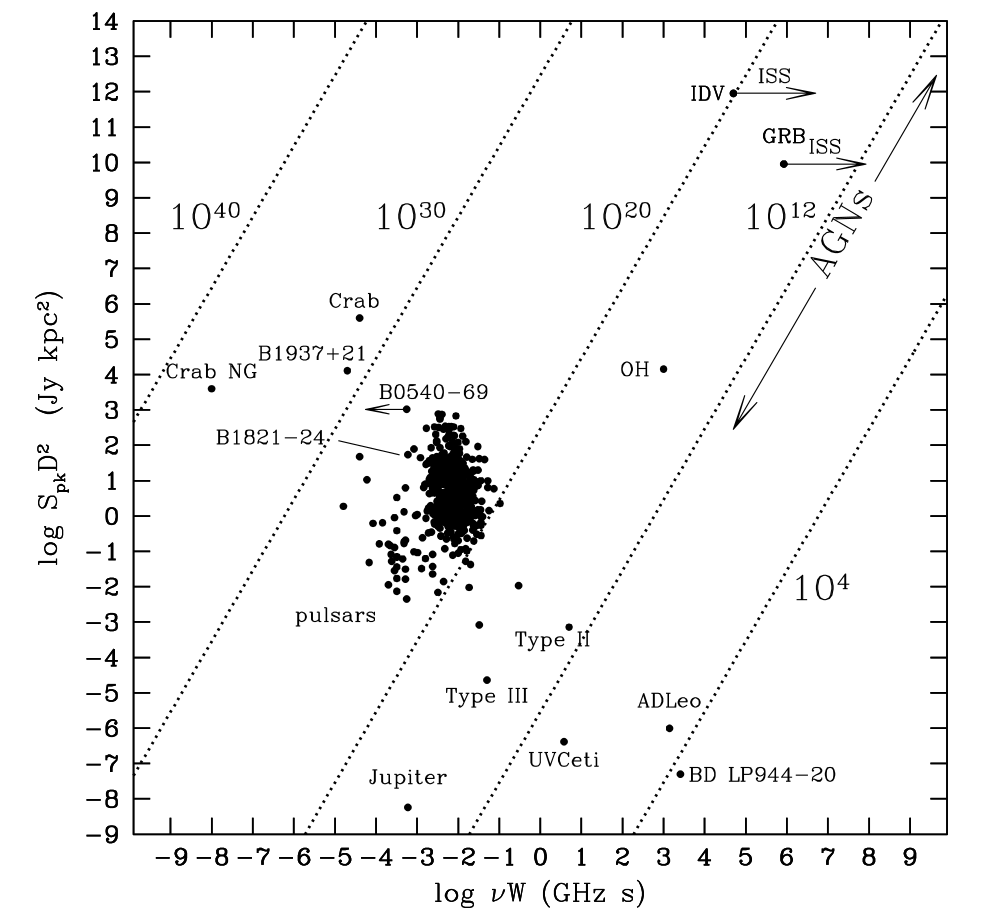
\includegraphics[width=5cm]{Flux.png} 
\end{figure}
As the Spectrum index might shows the high frequency will exist more energy, and this successful detection, It's an interesting things to start survey for FRB at higher frequency band.\\



If we have enough observe time, looking the other telescope might also an interesting things. Maybe that will give us a new understanding for FRB or test the theory that FRB is Giant Pulse from Pulsar. 
\subsection{2-D FFT Algorithm }
I got simple math analysis about 2D-FFT method. If we have a straight line $y=ax +b$, after 2D FFT:
\begin{equation} \begin{aligned}
&\int_{-\infty}^{+\infty}\int_{-\infty}^{+\infty}\delta(ax+b-y)e^{-i2\pi(ux+vy)}dxdy
\\ &= \int_{-\infty}^{+\infty}e^{-i2\pi(ux+v(ax+b))}dx
\\ &= \int_{-\infty}^{+\infty}e^{-i2\pi(u+av)x}dx \cdot e^{-i2\pi vb}
\\ &=\delta(u+av)\cdot e^{-i2\pi vb}
\end{aligned}
\end{equation}
In $(u,v)$ map ,straight line will become $v=-\frac{1}{a} x$, The b will be the module factor in $e^{-i2\pi vb}$.  
I got some straight width analysis, please see the PPT attached in E-mail.\\

In last Email, I found the interpolation in polar coordinate transform will bring a disaster time  consuming when data matrix got larger. When I almost give up ,I found a new way to search straight line according to angle,  we might not need to transform the map into polar coordinate , we could calculate the angle of each pixel, then using a histogram with weight of data to do this. This will have a high speed even at larger matrix. 

\section{Question Left}
I have started to compose paper about 2-D FFT algorithm. The angle resolution is not the problem brought by $\delta $DM, Actully it is not so important as the simulate Data test, Now I use $arctan(1 / $len(Data))  as the agnle resolution.  I want to discuss with you about G.White Noise after 2-D FFT. It should still be GWN, but they have real and imaginary two parts. the summation along angle will not become exact zero. \\
\\If we sum along angle directly with complex data after 2D FFT, the periodical will vanish from real and imaginary part, but if we sum the absolute data, the GWN will contribute to signal. 
\begin{figure}
\center
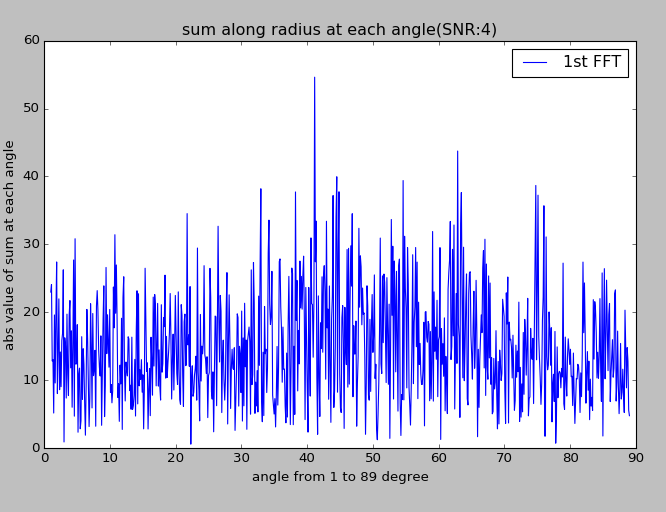
\includegraphics[width=8cm]{3.png}
\caption{Complex Data Sum}
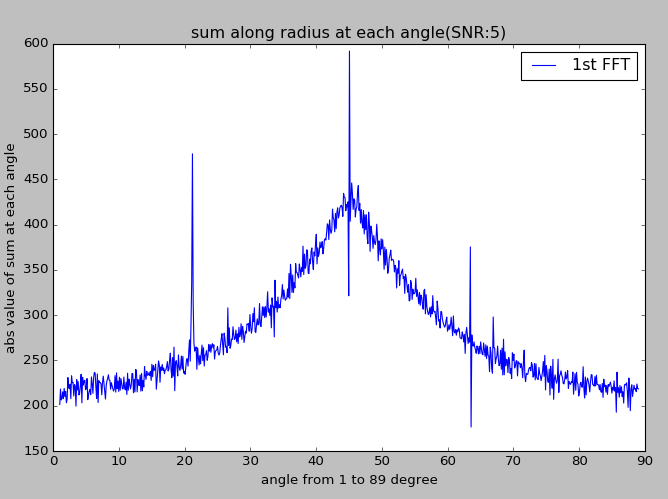
\includegraphics[width=8cm]{1.png}
\caption{Absolute Data Sum,0.11}
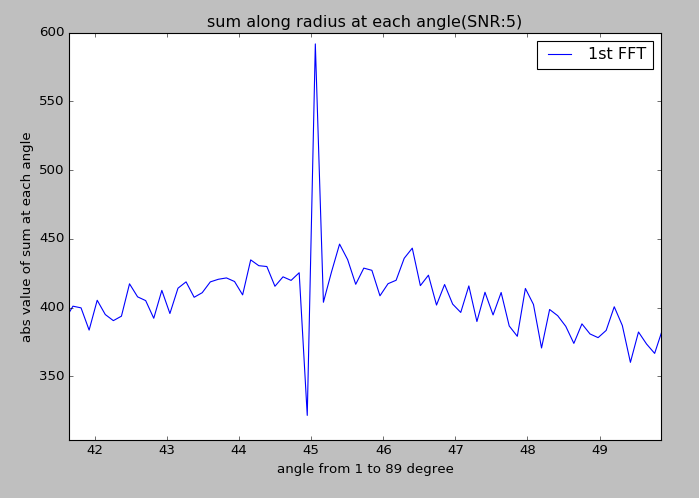
\includegraphics[width=6cm]{2.png}
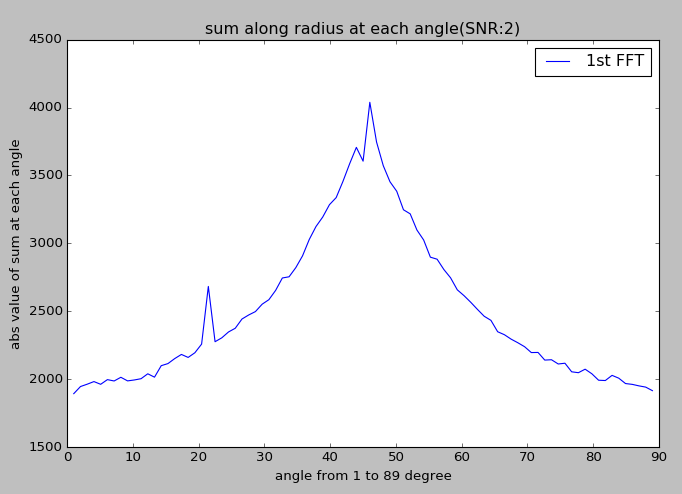
\includegraphics[width=6cm]{4.png}

\end{figure}

\end{document}

